\chapter{多目标Pareto优化分析}\label{chap:optimization}

参数化研究揭示了四个几何变量对各评价指标的单因素影响规律。然而，工程设计问题的本质是多目标权衡：同时追求高基底接触压力、低剪切应力、高压力传递效率与低泵送能耗，这些目标之间往往存在相互制约关系，无法通过单一参数调整同时满足所有需求。识别工程问题中需要完成的目标并将其按照紧迫性进行排序，最终通过多目标分析体系寻找一个满足多个要求的最优解，才能在实际的工程问题中找到一个权衡利弊的答案。为此，本章构建多目标Pareto优化分析框架，系统识别各目标之间的权衡关系，确定可行参数空间内的最优设计方案。

\section{多目标优化框架}

\subsection{设计变量与约束条件}

本研究的优化设计变量为四个几何参数，构成设计向量：
\begin{equation}\label{eq:design-vector}
  \mathbf{x} = (TL, \theta, L, \alpha) \in [30, 70] \times [15°, 60°] \times [10, 40] \times [0°, 20°].
\end{equation}
各变量的物理含义与取值范围见\cref{tab:5.1}。

\begin{table}[!htb]
  \centering
  \caption{设计变量定义与约束汇总表}\label{tab:5.1}
  \renewcommand{\arraystretch}{1.3}
  \begin{tabular}{cllll}
    \toprule
    \textbf{变量} & \textbf{物理含义} & \textbf{下界} & \textbf{上界} & \textbf{单位} \\
    \midrule
    $TL$     & 整形板长度    & 30 & 70           & mm \\
    $\theta$ & 喷嘴收缩角    & 15 & 60           & ° \\
    $L$      & 喷嘴竖直高度  & 10 & 40           & mm \\
    $\alpha$ & 整形板倾斜角  & 0  & 20（受$H$约束） & ° \\
    \bottomrule
  \end{tabular}
\end{table}

优化问题受到以下几何可行性约束的限制。整形板出口处的层高$H$由\cref{chap:parametric}第\ref{sec:alpha-influence}节推导的解析关系决定，其需满足：
\begin{equation}\label{eq:H-constraint}
  5~\text{mm} \leq H = Z_0 - TL \cdot \sin(\alpha) \leq 20~\text{mm},
\end{equation}
其中下界$H_{min} = 5$~mm保证沉积层具有最小可行厚度，上界$H_{max} = 20$~mm对应整形板完全水平（$\alpha = 0°$）时的层高上限。该约束本质上是对$\alpha$的上界施加了依赖于$TL$的动态限制。在最严苛情况下（$TL = 70$~mm），$\alpha$的解析上界为：
\begin{equation}\label{eq:alpha-max-strict}
  \alpha_{max} = \arcsin\left( \frac{Z_0 - H_{min}}{TL_{max}} \right) = \arcsin\left( \frac{22 - 5}{70} \right) = 14.06°.
\end{equation}
\cref{fig:5.1}在$\alpha$-$TL$参数平面内直观展示了几何可行域的边界。可以看出，随$TL$增大，可行的$\alpha$上界单调降低，呈现出整形板长度与倾斜角之间的固有几何耦合关系。图中同时标注了全部CFD工况点的位置，其中位于红色不可行区的B1-4工况（$\alpha = 20°$，$TL = 50$~mm，$H = 4.90$~mm）被排除出优化可行域。

\begin{figure}[!htb]
  \centering
  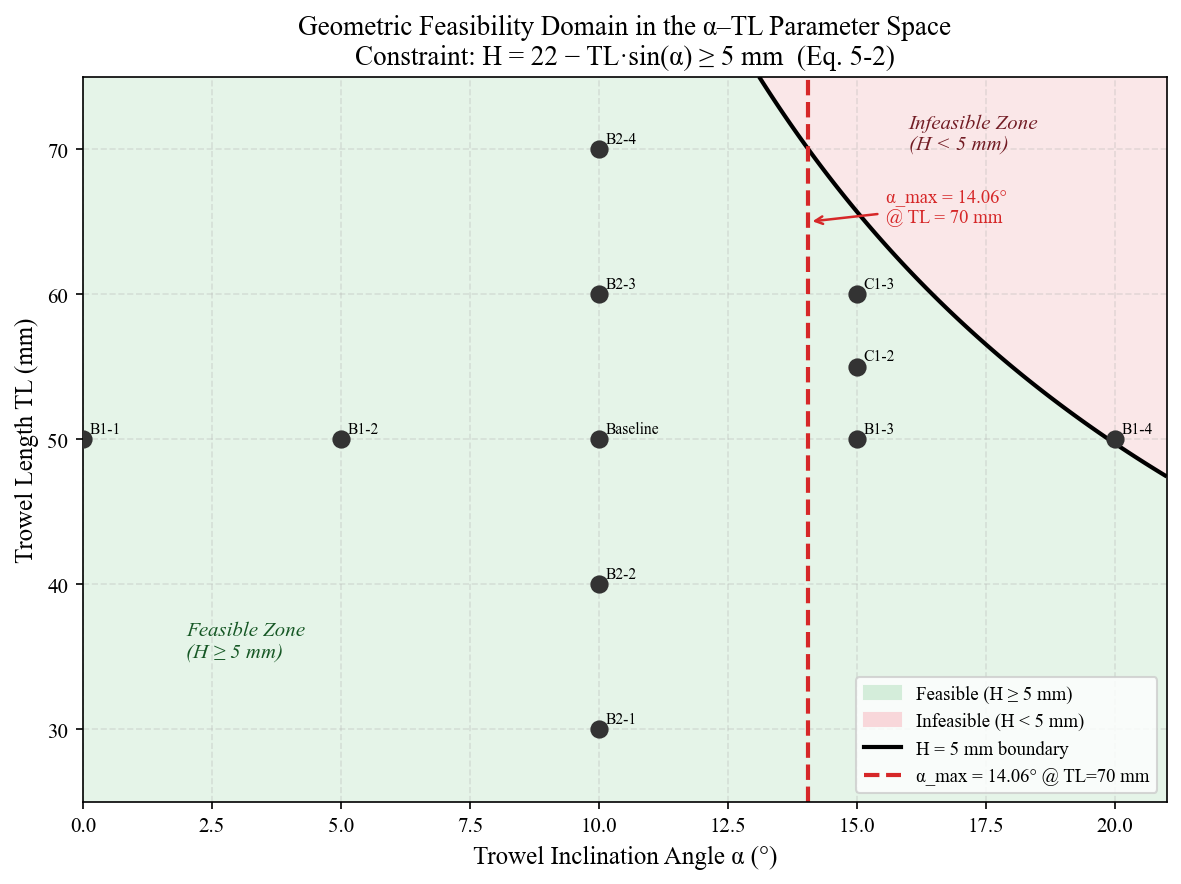
\includegraphics[width=0.8\textwidth]{figures/5.1.png}
  \caption{几何可行域示意图（$\alpha$-$TL$参数平面）}
  \label{fig:5.1}
\end{figure}

\subsection{五目标优化问题定义}

本研究将优化问题统一表述为最小化问题。对于原本需要最大化的目标，通过取负值将其转化为最小化形式。

本课题主要研究了两个优化问题。四目标优化平衡了基底面压力、喷嘴出口截面壁面剪切应力、压力传递效应与压力非均匀性指数，是在已有数据集的基础上进行目标简化，与此同时权衡重要性能、经济指标的结果。四目标优化问题的数学表述为：
\begin{equation}\label{eq:4-obj}
  \min_{\mathbf{x}} F(\mathbf{x}) = (-P_{sub,AWA},\ WSS_{nozzle},\ -\eta_p,\ UI).
\end{equation}

五目标优化是对四目标框架的重要扩展，将作为泵送能耗的代理指标$P_{inlet}$纳入其中。过高的泵送压力不仅增加能耗，还对泵送设备的密封性和使用寿命提出更高要求。在四目标框架中，$P_{inlet}$未被显式约束，优化器可能给出需要极高泵送压力的方案；纳入第五目标后，优化框架能够明确量化为获得更高接触压力所需付出的泵送代价，从而为工程决策提供更完整的信息。五目标优化问题的数学表述为：
\begin{equation}\label{eq:5-obj}
  \min_{\mathbf{x}} G(\mathbf{x}) = (-P_{sub,AWA},\ WSS_{nozzle},\ -\eta_p,\ UI,\ P_{inlet}).
\end{equation}

各目标的物理定义、优化方向及工程意义总结在\cref{tab:5.2}中。

\begin{table}[!htb]
  \centering
  \caption{优化目标定义、方向与工程意义汇总表}\label{tab:5.2}
  \renewcommand{\arraystretch}{1.3}
  \begin{tabular}{lllll}
    \toprule
    \textbf{目标} & \textbf{定义} & \textbf{方向} & \textbf{内化方向} & \textbf{工程意义} \\
    \midrule
    $f_1 = -P_{sub,AWA}$ & 基底接触压力     & 最大化 & 最小化 & 层间粘结强度 \\
    $f_2 = WSS_{nozzle}$ & 喷嘴剪切应力     & 最小化 & 最小化 & 材料损伤与磨损 \\
    $f_3 = -\eta_p$      & 压力传递效率     & 最大化 & 最小化 & 泵送经济性 \\
    $f_4 = UI$           & 压力非均匀性     & 最小化 & 最小化 & 层间质量均匀性 \\
    $f_5 = P_{inlet}$    & 入口压力         & 最小化 & 最小化 & 泵送能耗代理 \\
    \bottomrule
  \end{tabular}
\end{table}

\section{代理模型建立}

遗传算法需要在优化过程中需要对目标函数进行数万次评估，而三维几何建模与CFD分析需要很大的计算能力与时间，这让代理直接调用CFD仿真在计算成本上基本不可行。本课题于是建立了一个能够快速预测目标函数值的代理模型（Surrogate Model），以完成后续分析。

\subsection{多项式RSM（2阶Ridge回归）}

选用2阶多项式响应面方法（Response Surface Methodology，RSM）配合Ridge正则化（正则化系数$\lambda = 1.0$）作为代理模型。2阶多项式RSM的基函数展开形式为：
\begin{equation}\label{eq:rsm}
  \hat{f}(\mathbf{x}) = \beta_0 + \sum_i \beta_i x_i + \sum_i \beta_{ii} x_i^2 + \sum_{i<j} \beta_{ij} x_i x_j.
\end{equation}
对于4个设计变量，该模型共包含：4个线性项、4个二次项、6个交叉项，1个截距项，共计15个系数。考虑到本研究可用的可行工况数量为17个，2阶多项式RSM与数据规模匹配较好，在保证拟合能力的同时不至于严重过拟合。

在模型选择方面，本课题同时评估了高斯过程回归（Gaussian Process Regression，GPR）和梯度提升回归（Gradient Boosting Regression，GBR）方法。GPR在理论上具有较强的非线性拟合能力，但在仅17个数据点的条件下，其留一法交叉验证（LOO-CV）得到的$R^2$仅为0.37，泛化能力不稳定；GBR属于集成学习方法，对小样本同样容易出现过拟合。相比之下，2阶多项式RSM配合Ridge正则化在小样本工程参数优化中具有更稳定的泛化表现，且系数具有明确的物理解释性（各变量的线性项、二次项系数直接反映其对目标函数的影响方向与强度），因此选用该方法作为本研究的代理模型。

\subsection{留一法交叉验证（LOO-CV）}

为客观评估代理模型的预测精度，采用留一法交叉验证（Leave-One-Out Cross-Validation，LOO-CV）对各目标的代理模型进行验证。LOO-CV能够在不额外消耗CFD计算资源的前提下，对小样本代理模型的泛化能力给出无偏估计。五目标代理模型的LOO-CV结果汇总于\cref{tab:5.3}，对应的预测值与实际值散点图见\cref{fig:5.2}。预测模型的集成多项式RSM响应面如\cref{fig:5.3}所示。

\begin{figure}[!htb]
  \centering
  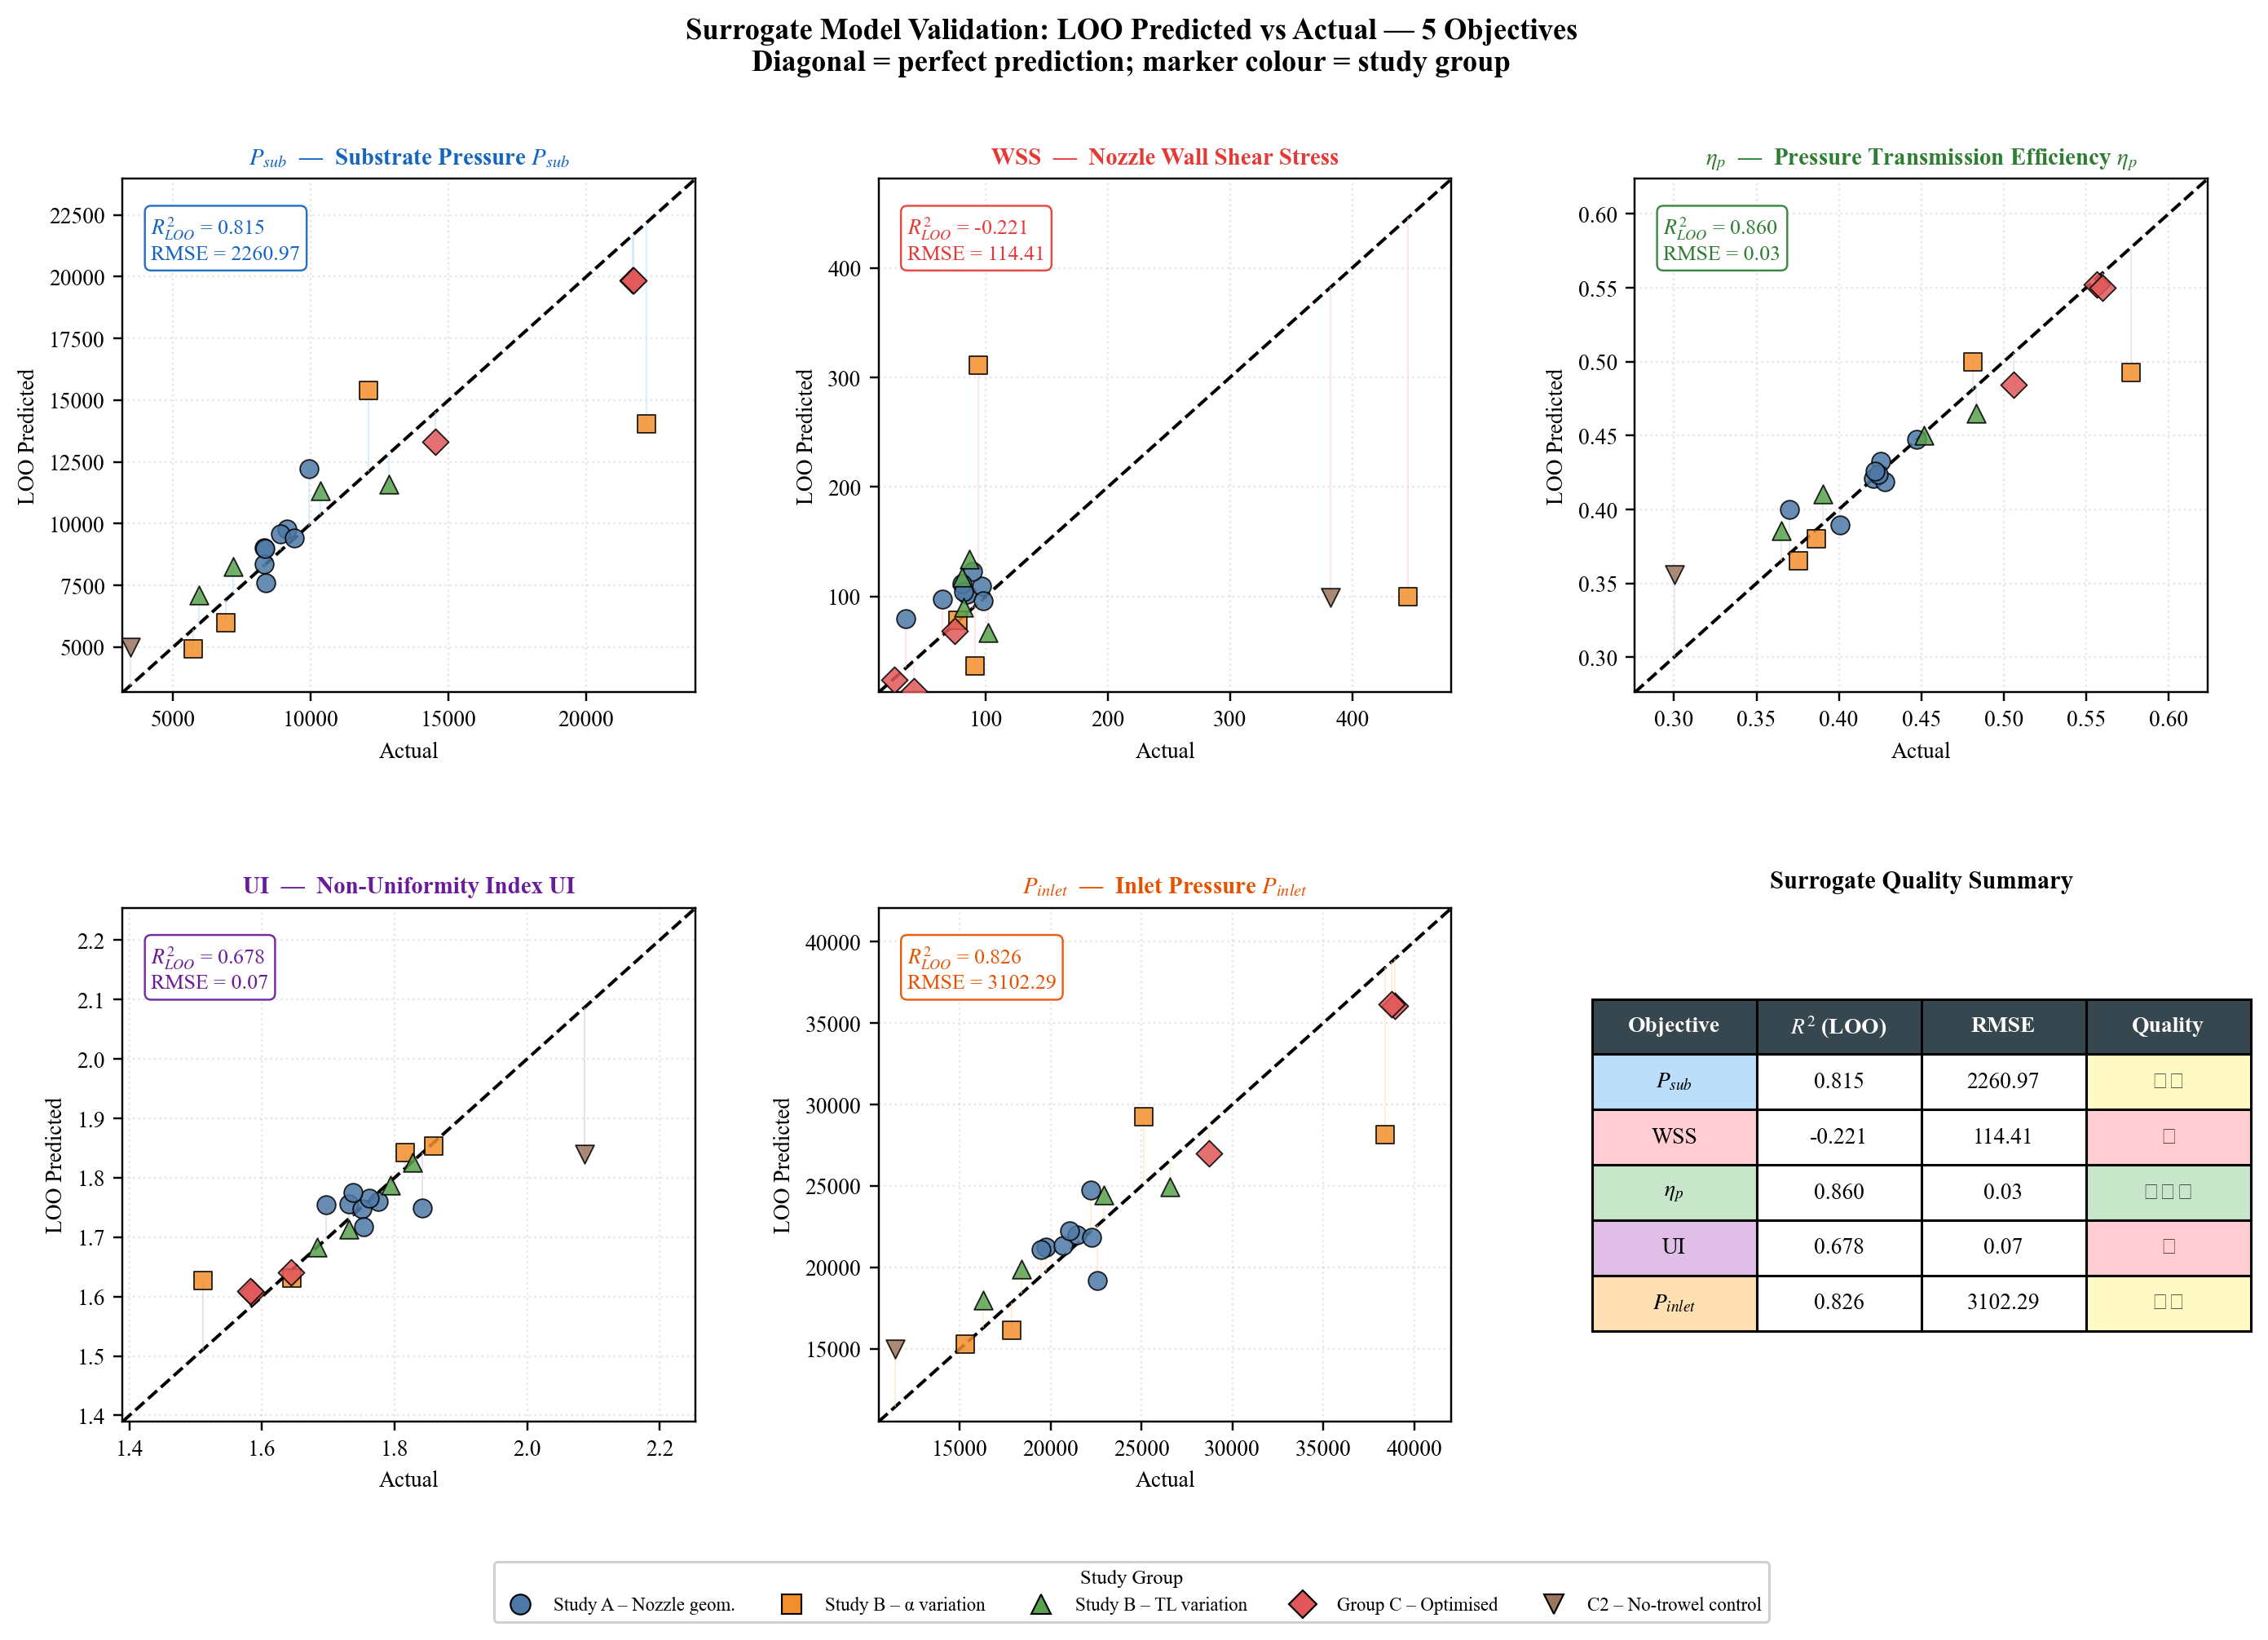
\includegraphics[width=0.9\textwidth]{figures/5.2.png}
  \caption{各目标LOO预测值与实际值对比散点图}
  \label{fig:5.2}
\end{figure}

\begin{figure}[!htb]
  \centering
  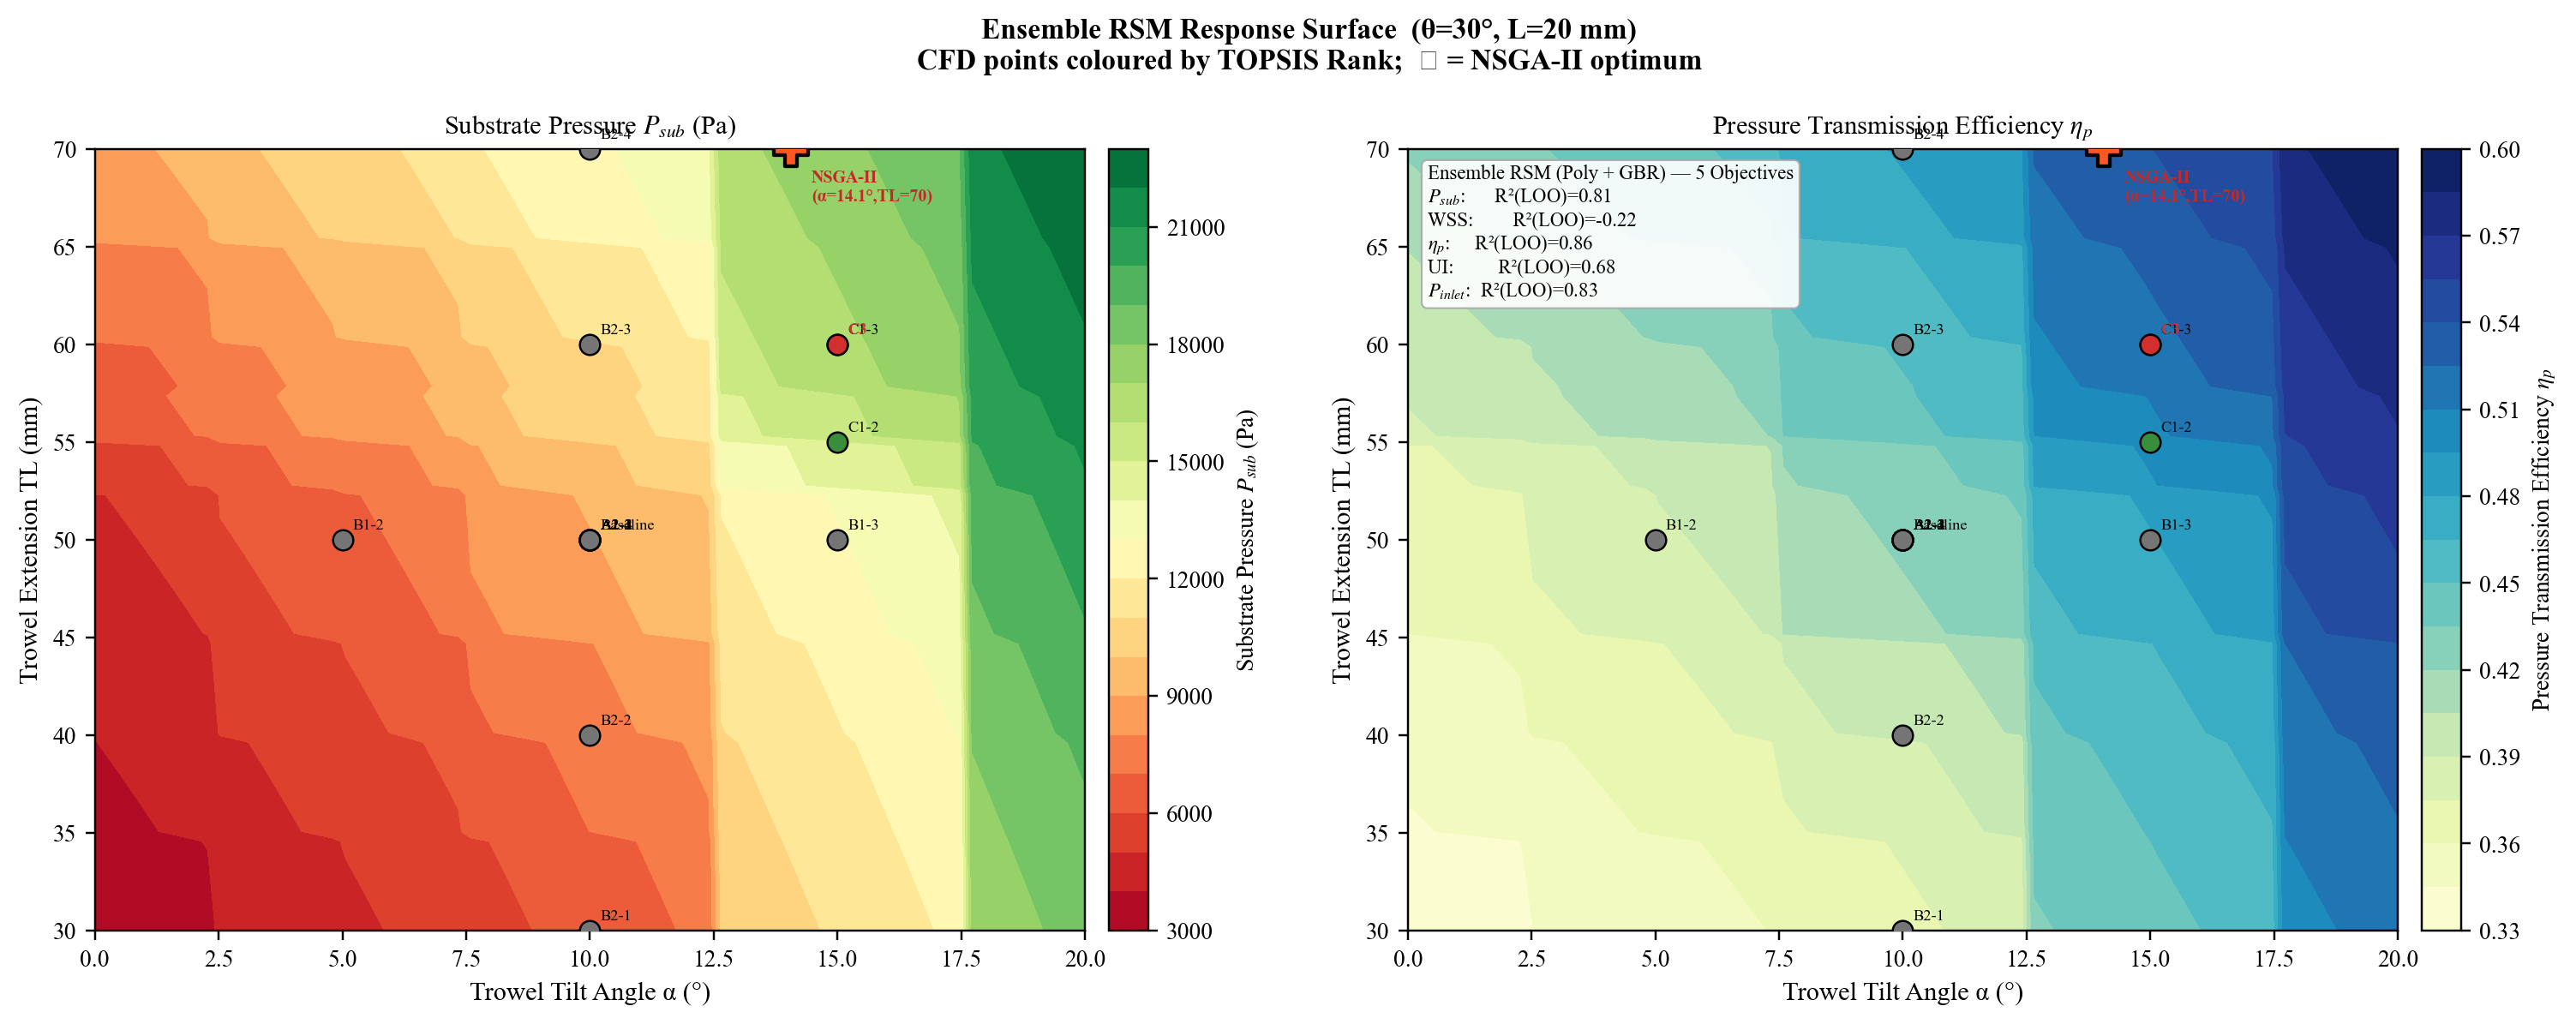
\includegraphics[width=0.95\textwidth]{figures/5.3.png}
  \caption{集成多项式RSM响应面（左）、CFD数据点与NSGA-II最优点（右）}
  \label{fig:5.3}
\end{figure}

\begin{table}[!htb]
  \centering
  \caption{代理模型LOO-CV结果汇总}\label{tab:5.3}
  \renewcommand{\arraystretch}{1.3}
  \begin{tabular}{lcccc}
    \toprule
    \textbf{目标} & \textbf{方法} & $R^2$(LOO) & \textbf{RMSE} & \textbf{可信度评级} \\
    \midrule
    $P_{sub,AWA}$    & Poly RSM & 0.815  & 2260.97 & 强 \\
    $WSS_{nozzle}$   & Poly RSM & -0.221 & 114.41  & 低 \\
    $\eta_p$         & Poly RSM & 0.860  & 0.03    & 较强 \\
    $UI$             & Poly RSM & 0.678  & 0.07    & 一般 \\
    $P_{inlet}$      & Poly RSM & 0.826  & 3102.29 & 较强 \\
    \bottomrule
  \end{tabular}
\end{table}

由结果可见，各目标代理模型的预测质量存在明显差异。$P_{sub,AWA}$的代理模型表现最好，说明代理模型能够较为可靠地捕捉基底压力随参数变化的趋势。$\eta_p$的代理模型质量居中，由于$\eta_p = P_{sub}/P_{inlet}$，其变化趋势与$P_{sub}$高度相关（$r = 0.962$），代理模型能够对其进行合理预测。

$WSS_{nozzle}$的代理模型质量最差，LOO-CV得到的$R^2$为负值，说明代理模型的预测能力甚至不及简单均值预测。这一异常结果的根本原因在于数据中存在严重的异常点：B1-1工况（$\alpha = 0°$）的$WSS_{nozzle} = 445.5$~Pa，约为其他工况平均值的5.6倍，这一极端值严重扭曲了代理模型的拟合，使模型既无法准确拟合正常工况，也无法正确预测异常工况。$UI$的代理模型同样表现较差，主要原因可能在于$UI$对几何参数的响应关系的复杂性，模型很难在17个数据点的条件下完整刻画4个主效应项和6个交叉项。

\subsection{模型局限性}

本课题建立的代理模型具有以下的局限性，需要在根据代理模型优化决策时慎重考虑：

（1）数据规模对泛化能力的限制。本研究仅有17个可行CFD工况，而代理模型需要在4维参数空间中进行插值与外推。数据点的分布遵循单因素变化原则，参数空间的``角落''（如高$TL$、高$\theta$、高$\alpha$的组合）缺乏直接CFD数据，代理模型在这些区域的预测可信度较低。

（2）$L$变量信息不足。Pearson相关分析已证明$L$对$P_{sub,AWA}$的影响在统计上不显著（$r = -0.038$，$p = 0.873$）。在代理模型中，$L$的变化几乎不改变任何目标函数的预测值，这意味着代理模型对$L$这个维度基本无感，NSGA-II在$L$方向的优化结果（$L = 40$~mm）本质上是在一个噪声主导的维度上搜索，物理意义有限，不宜据此对$L$参数作出工程推荐。

（3）$WSS_{nozzle}$代理模型不可用于定量预测。鉴于$WSS_{nozzle}$代理模型的负$R^2$，NSGA-II基于该模型对$WSS_{nozzle}$的优化结果仅具有方向性参考价值（即``更小的$\alpha$和$\theta$有利于降低WSS''的趋势），而不能作为绝对值预测的依据。

在后续对课题的深度研究和完善过程中，可以通过拉丁超立方抽样等的种种空间填充方法增加CFD工况，以提升代理模型的空间覆盖度，增加代理模型的可信度。

\section{TOPSIS综合排名}

\subsection{归一化加权评分方法}

在对17个可行工况进行综合排名时，采用TOPSIS（Technique for Order Preference by Similarity to Ideal Solution）思路的线性加权归一化评分方法。具体步骤为：将五个目标的实测值分别进行Min-Max归一化，使各目标均映射至$[0, 1]$区间，方向统一为归一化值越小越优，对于需要最大化的目标，归一化时取反；随后以等权重$w_i = 0.2$对归一化后的五个目标进行加权求和，得到复合评分：
\begin{equation}\label{eq:topsis}
  S_{composite} = \sum_{i=1}^{5} w_i \cdot f_i^{norm}, \quad w_i = 0.2.
\end{equation}
复合得分越小，表明该工况在五个目标上的综合表现越优。

此处等权重计算不同目标的决定，是在缺乏明确工程优先级信息的情况下对各目标不偏不倚的处理方式。但是在实际工程应用中，不同工程在不同时段会产生不同的目标与优先级，需要根据具体需求对权重进行调整。

\subsection{排名结果}

17个可行工况的TOPSIS综合排名结果见\cref{fig:5.4}与\cref{tab:5.4}。

\begin{table}[!htb]
  \centering
  \caption{TOPSIS工况排名表}\label{tab:5.4}
  \renewcommand{\arraystretch}{1.3}
  \begin{tabular}{ccccccccc}
    \toprule
    \textbf{排名} & \textbf{工况} & $TL$ & $\theta$ & $\alpha$ & $P_{sub,AWA}$ & $WSS_{nozzle}$ & $\eta_p$ & $UI$ \\
    \midrule
    1 & C3   & 60 & 60° & 15° & 21702 & 25.1  & 0.560 & 1.582 \\
    2 & C1-3 & 60 & 60° & 15° & 21677 & 41.1  & 0.557 & 1.585 \\
    3 & C1-2 & 55 & 30° & 15° & 14525 & 74.7  & 0.506 & 1.644 \\
    4 & B1-3 & 50 & 30° & 15° & 12081 & 77.1  & 0.481 & 1.645 \\
    5 & B2-4 & 70 & 30° & 10° & 12833 & 102.1 & 0.483 & 1.683 \\
    \bottomrule
  \end{tabular}
\end{table}

\begin{figure}[!htb]
  \centering
  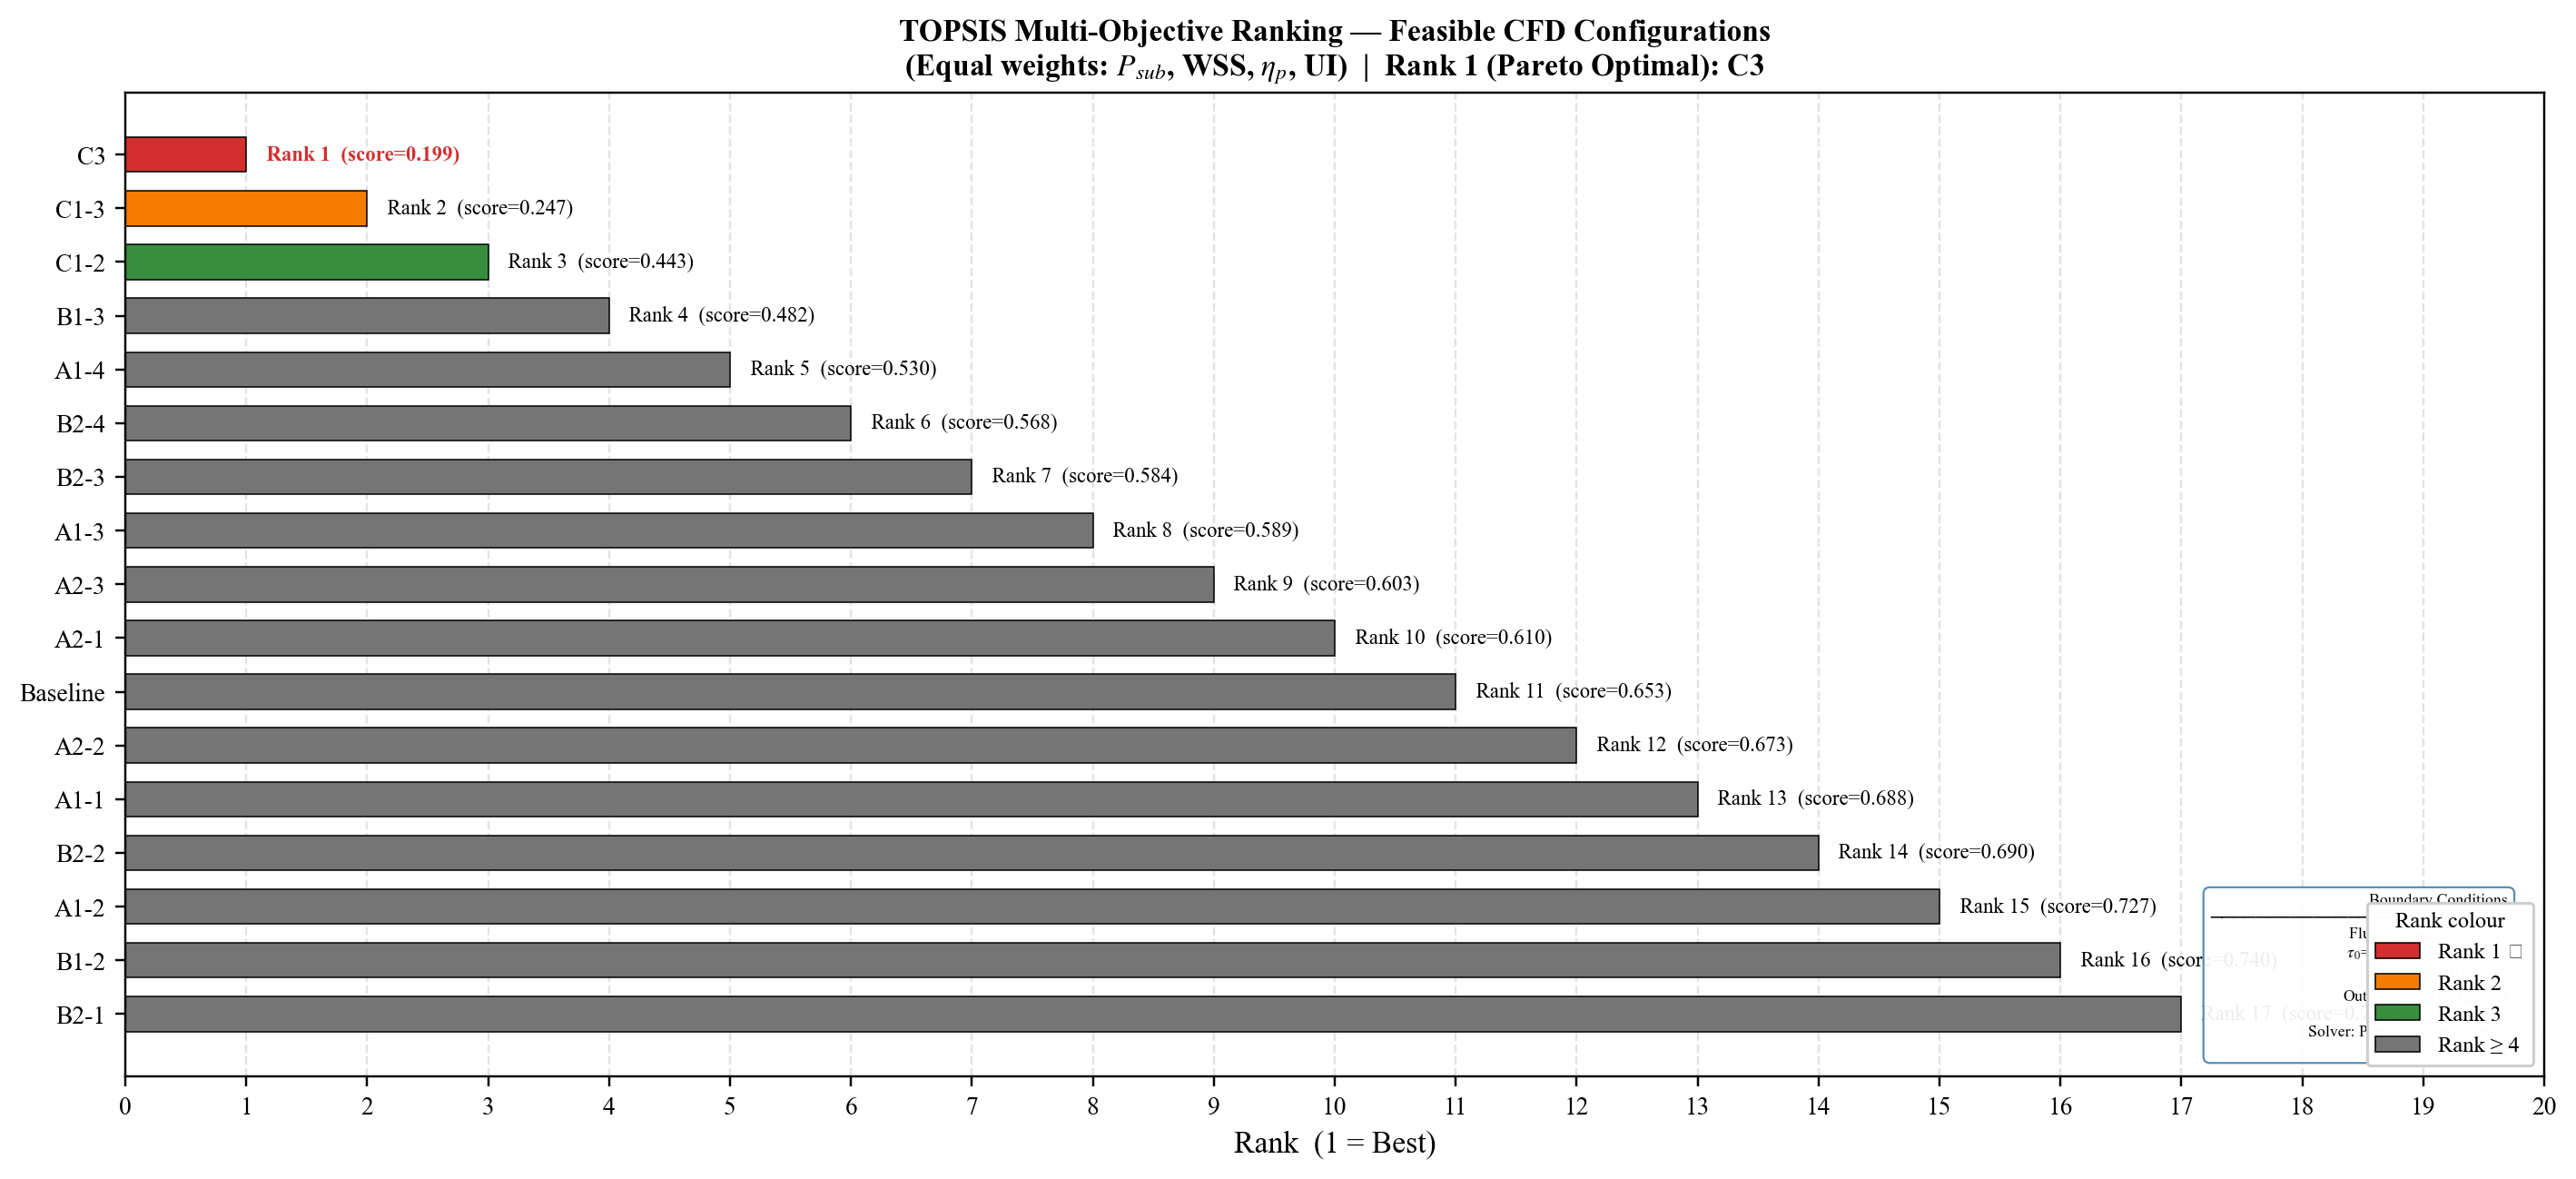
\includegraphics[width=0.8\textwidth]{figures/5.4.png}
  \caption{TOPSIS综合排名水平柱状图}
  \label{fig:5.4}
\end{figure}

C3工况（$TL = 60$~mm，$\theta = 60°$，$L = 20$~mm，$\alpha = 15°$，含Fillet）以复合得分0.000排名第一，是本研究在五目标等权重框架下的综合最优配置。C1-3工况紧随其后（$S = 0.059$），两者参数完全相同，仅几何倒角处理有所不同。C3对C1-3的优势集中体现在$WSS_{nozzle}$指标上（25.1 vs 41.1 Pa，降低39\%），在其他四个目标上两者几乎无差异（$P_{sub}$差异$<0.1\%$，$\eta_p$差异$<0.6\%$）。这再次说明：几何倒角虽然对宏观压力场影响微乎其微，但其对喷嘴近壁剪切状态的改善足以在五目标等权重评分中拉开差距，确立C3的综合最优地位。

第3-5名（C1-2、B1-3、B2-4）均包含$\alpha = 15°$或$TL \geq 60$~mm，也进一步印证了\cref{chap:parametric}参数重要性排序的结论，即$\alpha$和$TL$是对综合性能贡献最大的两个参数。排名靠后的工况（如A1-2、B1-2、B2-1等）共同特点是接触压力较低或$\eta_p$较小，说明在等权重评分下，接触压力维度的相对劣势难以被其他目标的优势所弥补。在实际工程运用中，排名与不同工况所产生的优势势必会随着权重与目标的不同而变化。

\section{Pareto Front支配分析}

\subsection{四目标Pareto Front分析}

Pareto支配分析是多目标优化中识别不可改进解的标准方法。若不存在任何其他可行解能够在所有目标上同时不差于该解、且至少在一个目标上严格优于该解，则称该解为Pareto最优解（Pareto-optimal solution），Pareto最优解的集合构成Pareto前沿。

在四目标框架（$f_1 = -P_{sub}$，$f_2 = WSS_{nozzle}$，$f_3 = -\eta_p$，$f_4 = UI$）下，对17个可行CFD工况进行穷举式Pareto支配判断，结果表明：C3是唯一的Pareto最优配置，在四维目标空间中不受任何其他工况的支配。

\cref{fig:5.5}展示了四对目标组合下的二维Pareto散点图。在所有子图中，C3均位于其他工况构成的散点群的前沿位置，直观验证了其Pareto最优性。

\begin{figure}[!htb]
  \centering
  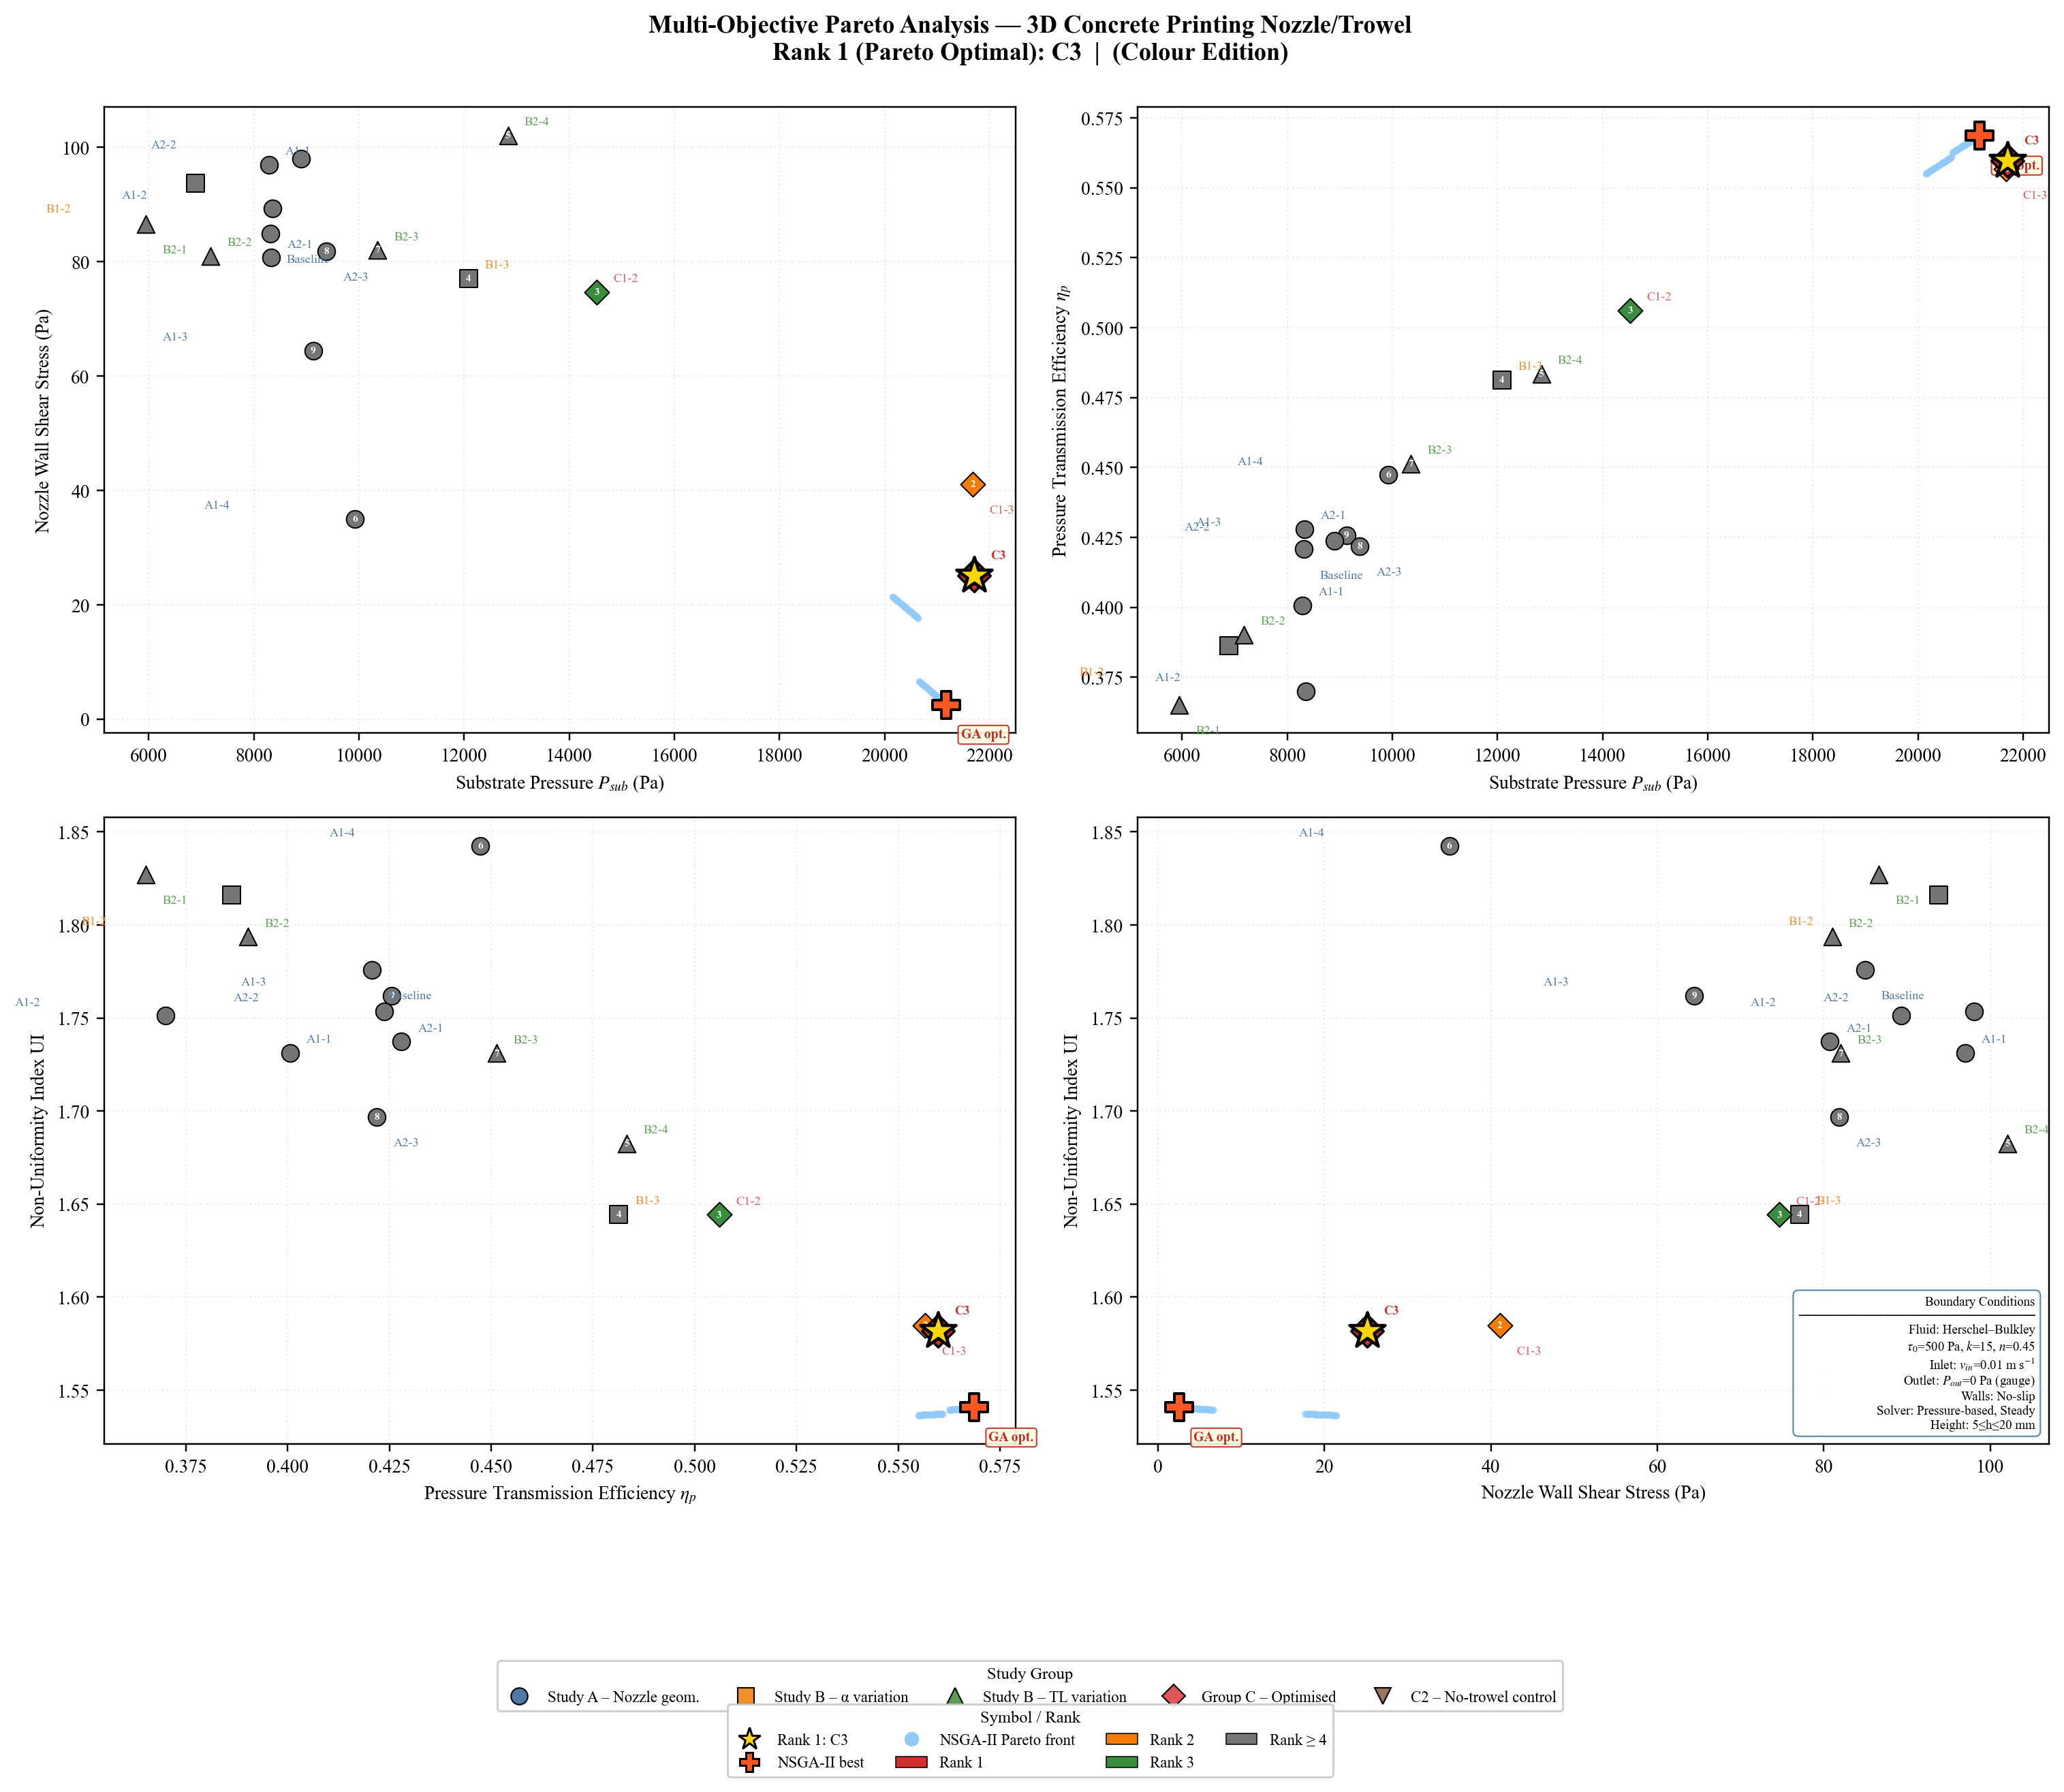
\includegraphics[width=0.95\textwidth]{figures/5.5.png}
  \caption{四目标Pareto散点图}
  \label{fig:5.5}
\end{figure}

次优工况C1-3在$P_{sub}$（21677 vs 21702 Pa，差0.1\%）、$\eta_p$（0.557 vs 0.560，差0.5\%）和$UI$（1.585 vs 1.582，差0.2\%）三个目标上与C3几乎无差异，但在$WSS_{nozzle}$（41.1 vs 25.1 Pa）上明显劣于C3，因此被C3严格支配。这一分析再次确认：在C1-3基础上增加几何倒角（C3）是一个严格的Pareto改进，在不损失任何其他目标性能的前提下，显著降低了喷嘴壁面剪切应力，体现了倒角作为几何优化手段的确定性价值。

\subsection{五目标Pareto Front分析与目标共线性}

将$P_{inlet}$纳入第五个优化目标后，Pareto格局发生了根本性变化：Pareto最优点从1个扩展至13个（占17个可行工况的76\%），大量低能耗工况（如B2-1、B1-2等）进入Pareto Front。最优点数量激增这一显著变化的根源在于$P_{inlet}$与$P_{sub,AWA}$之间的体现的高度共线性。20个CFD工况在$P_{inlet}$-$P_{sub,AWA}$散点图上的分布图如\cref{fig:5.6}所示。

\begin{figure}[!htb]
  \centering
  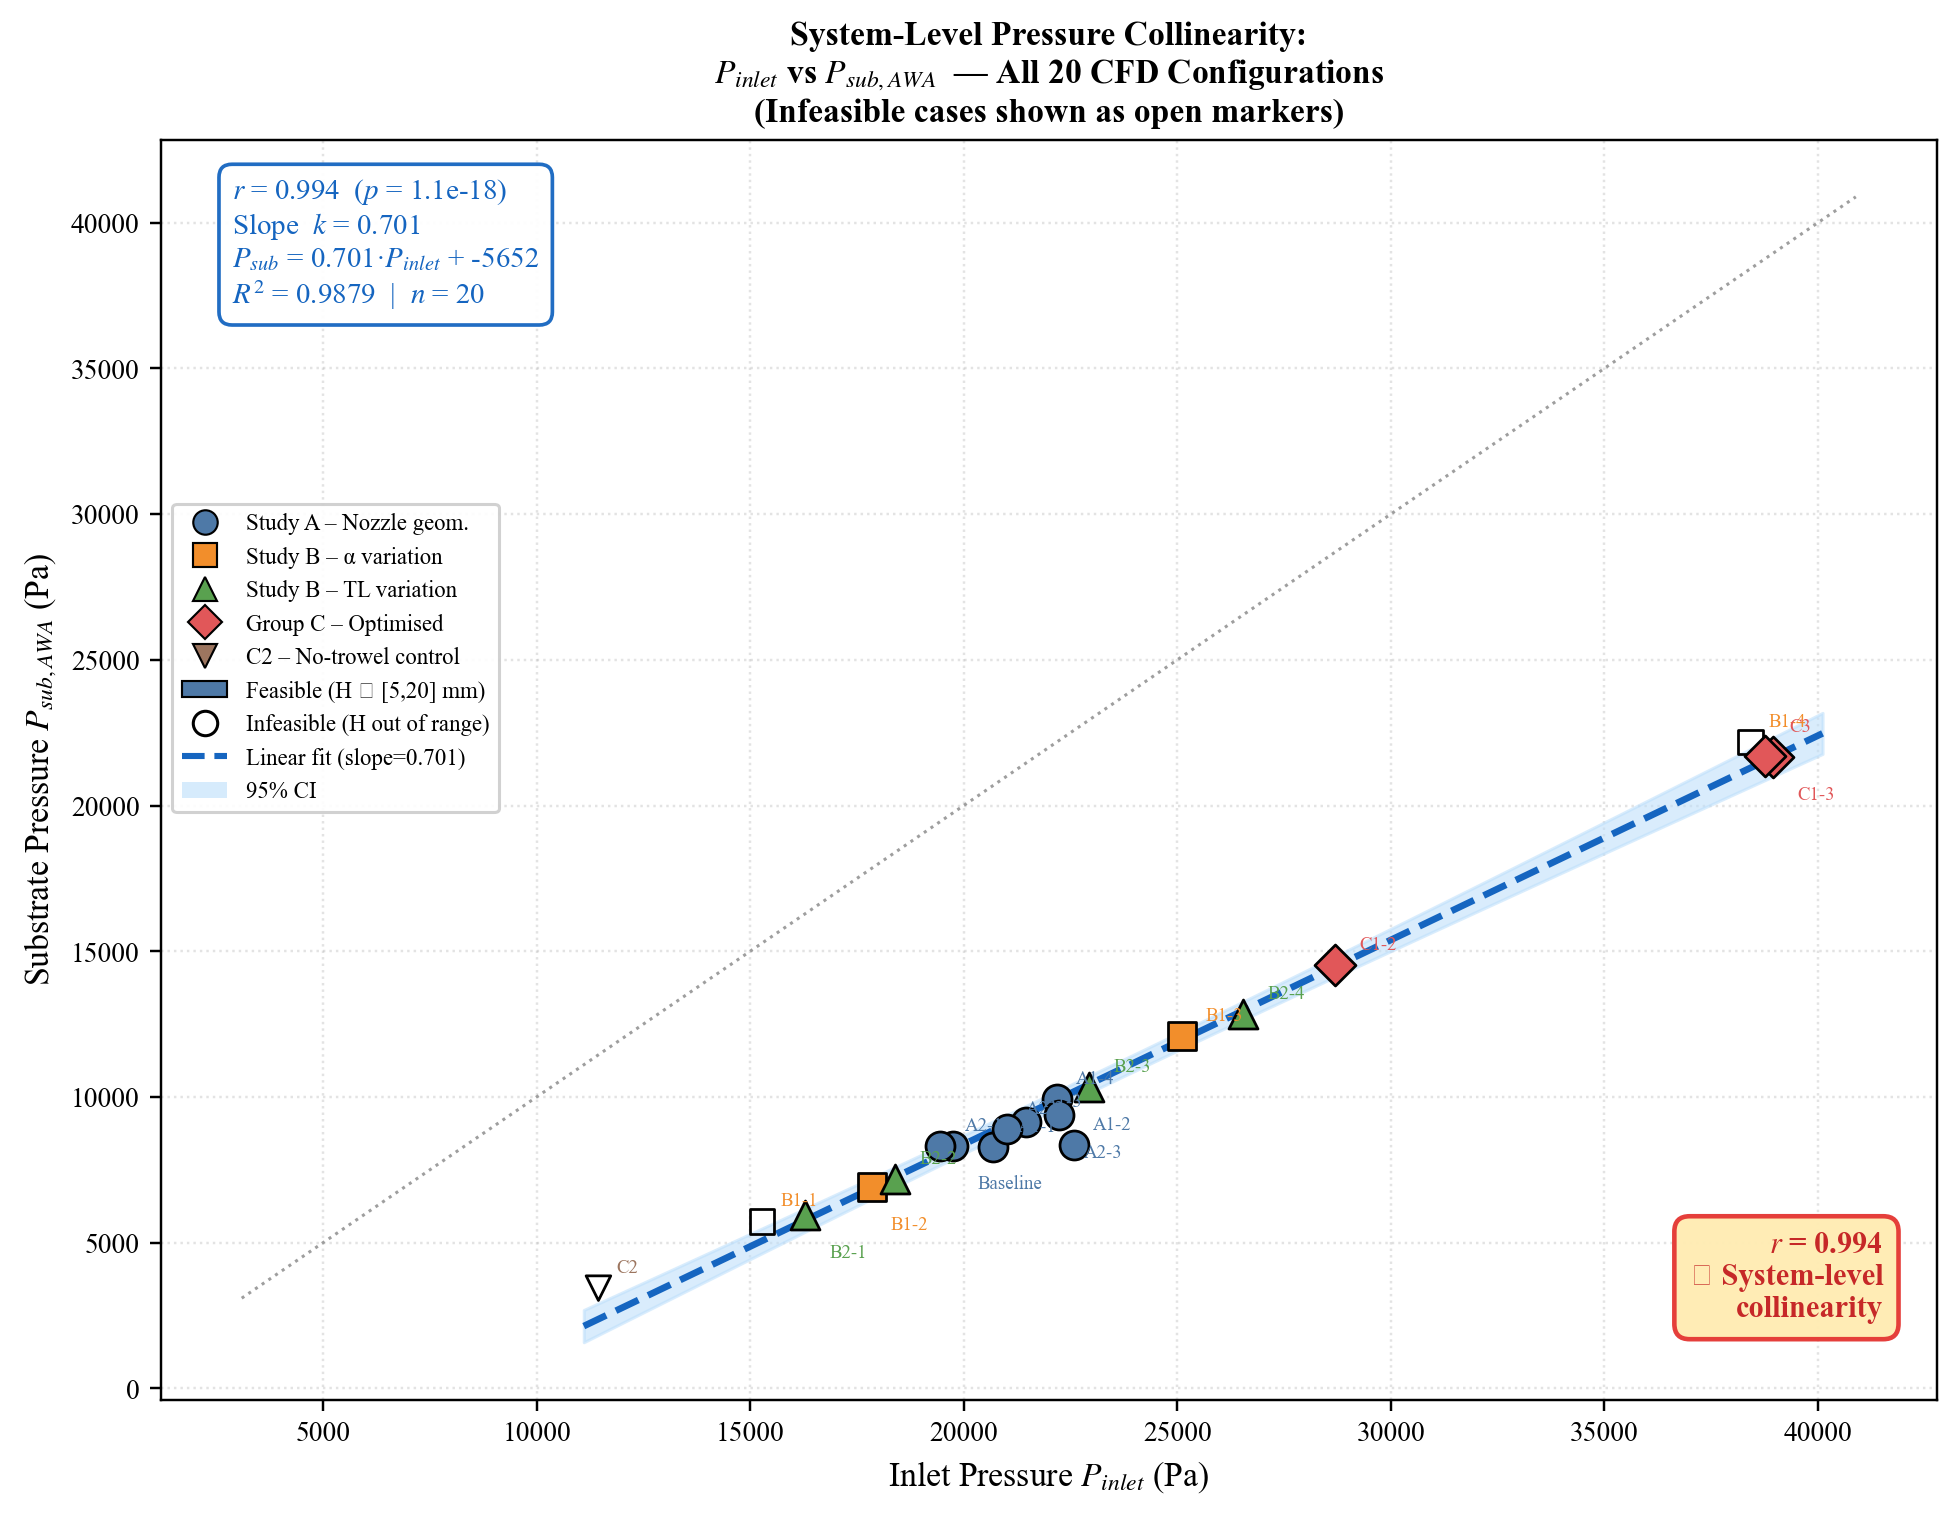
\includegraphics[width=0.75\textwidth]{figures/5.6.png}
  \caption{$P_{inlet}$--$P_{sub,AWA}$散点图}
  \label{fig:5.6}
\end{figure}

线性拟合结果表明：
\begin{equation}\label{eq:Pinlet-Psub}
  P_{inlet} \approx \frac{1}{\bar{\eta}_p} \cdot P_{sub,AWA} \approx 1.427 \cdot P_{sub,AWA},
\end{equation}
Pearson相关系数$r = 0.9879$（$p < 0.001$），20个工况的数据点几乎完美地排列在一条直线上。这一近乎确定性的线性关系揭示了本研究打印系统的一个基本物理规律：在当前喷嘴-整形板几何框架下，提升基底接触压力与增大泵送入口压力是等价的操作。系统的压力传递效率$\eta_p$在不同工况间的变异极小（约在0.37-0.58之间），几何参数的改变主要影响压力的绝对水平，而非传递效率本身。

\cref{tab:5.5}列出了主要目标对的Pearson相关系数。除$P_{inlet}$-$P_{sub}$的高度共线性外，结合\cref{fig:4.20}还可观察到：$\eta_p$与$P_{sub}$之间具有强正相关性（$r = 0.962$），而$UI$与$\eta_p$之间展现强负相关（$r = -0.901$）。这说明在本研究的参数空间内，五个目标并非独立，压实能力、剪切损伤、低能耗这三个目标基本涵盖了全部五个目标的信息。

\begin{table}[!htb]
  \centering
  \caption{主要目标对的Pearson相关系数表}\label{tab:5.5}
  \renewcommand{\arraystretch}{1.3}
  \begin{tabular}{lccccc}
    \toprule
                 & $P_{sub,AWA}$ & $WSS_{nozzle}$ & $\eta_p$ & $UI$    & $P_{inlet}$ \\
    \midrule
    $P_{sub,AWA}$  & 1.000  & -0.465 & 0.962  & -0.861 & 0.994  \\
    $WSS_{nozzle}$ & -0.465 & 1.000  & -0.534 & 0.629  & -0.518 \\
    $\eta_p$       & 0.962  & -0.534 & 1.000  & -0.901 & 0.953  \\
    $UI$           & -0.861 & 0.629  & -0.901 & 1.000  & -0.884 \\
    $P_{inlet}$    & 0.994  & -0.518 & 0.953  & -0.884 & 1.000  \\
    \bottomrule
  \end{tabular}
\end{table}

在五目标框架下，低接触压力但低泵送能耗的工况（如B2-1：$P_{sub} = 5944$~Pa，$P_{inlet} = 16277$~Pa）与高接触压力但高泵送能耗的工况（如C3：$P_{sub} = 21702$~Pa，$P_{inlet} = 38772$~Pa）处于同等的Pareto地位，因为两者各有所长，无法通过单一工况在所有五个目标上同时超越对方，而这也正是五目标分析所揭示的能耗-压实固有权衡关系的集中体现。工程师在实际打印系统设计中，需要根据泵送设备的压力能力和对层间粘结强度的具体要求，在Pareto Front上选取合适的工作点。

\section{NSGA-II多目标遗传算法优化}\label{sec:nsga2}

\subsection{NSGA-II算法设置}

NSGA-II（Non-dominated Sorting Genetic Algorithm II）是求解多目标优化问题的一种遗传算法，其核心特征是通过非支配排序与拥挤距离机制，在单次运行中同时生成分布均匀的Pareto Front近似解集，适合处理连续参数空间内的多目标工程优化问题。

本课题建立的NSGA-II遗传算法以建立多项式RSM代理模型作为目标函数评估器，每次函数评估的计算时间为毫秒量级，使算法能够在合理时间内完成$200 \times 300 = 60000$次函数评估。具体超参数设置见\cref{tab:5.6}。

\begin{table}[!htb]
  \centering
  \caption{NSGA-II算法参数设置}\label{tab:5.6}
  \renewcommand{\arraystretch}{1.3}
  \begin{tabular}{lll}
    \toprule
    \textbf{参数} & \textbf{设定值} & \textbf{说明} \\
    \midrule
    种群规模         & 200             & 4维参数空间覆盖 \\
    迭代代数         & 300             & 收敛性保证 \\
    交叉算子         & SBX             & 模拟二进制交叉 \\
    变异算子         & PM              & 多项式变异 \\
    随机种子         & 42              & 结果可重现 \\
    约束处理         & 惩罚函数        & 层高约束 $H \geq 5$~mm \\
    \bottomrule
  \end{tabular}
\end{table}

种群规模200能够为4维参数空间提供足够的多样性覆盖；模拟二进制交叉（SBX）和多项式变异（PM）是处理连续变量优化问题的标准算子；随机种子固定为42确保结果可重现；层高约束通过惩罚函数处理，对不满足$H \geq 5$~mm的个体施加大惩罚值，使其在非支配排序中被自动淘汰。这些关键设置可以保证NSGA-II在课题特定的五目标框架下发挥较优解析能力。

\subsection{NSGA-II Pareto Front结果}

\cref{fig:5.7}给出了NSGA-II生成的Pareto Front（约200个解）与17个CFD数据点在四对目标组合下的叠加图。

\begin{figure}[!htb]
  \centering
  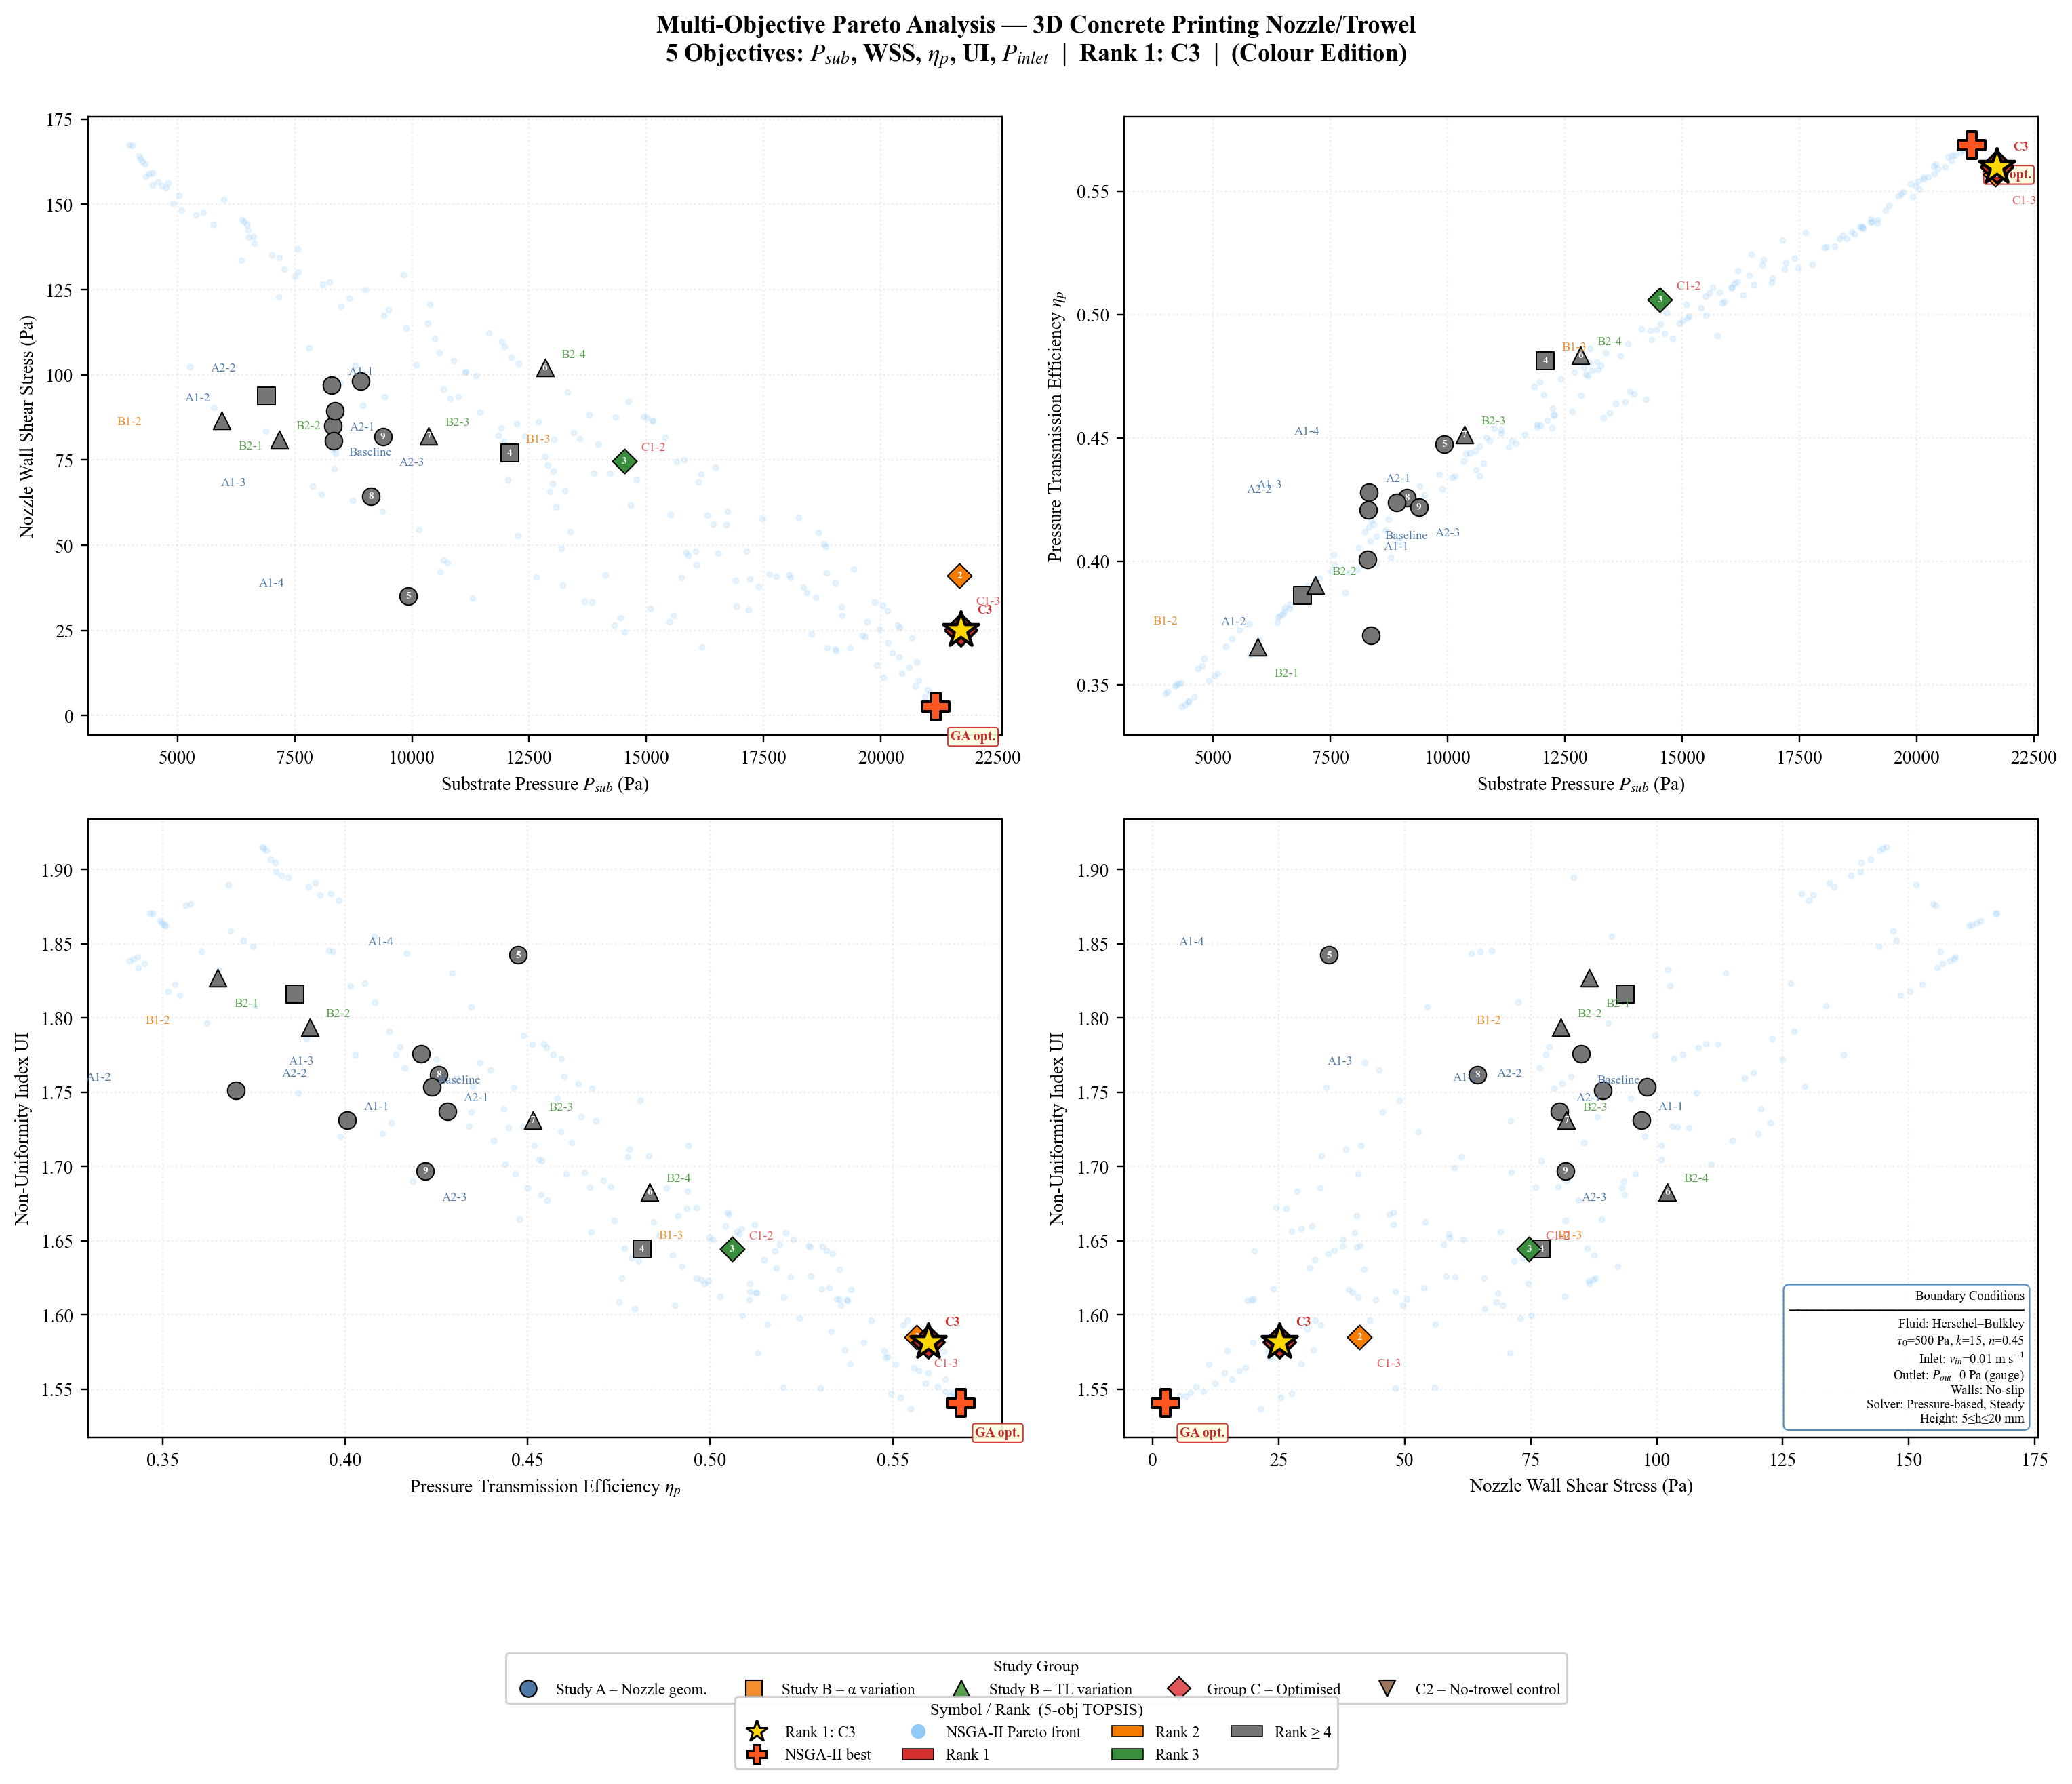
\includegraphics[width=0.95\textwidth]{figures/5.7.png}
  \caption{NSGA-II Pareto Front结果散点图}
  \label{fig:5.7}
\end{figure}

由图可见，NSGA-II生成的Pareto Front在$P_{sub}$-$WSS$和$P_{sub}$-$\eta_p$空间中均呈现出连续平滑的曲线形态，清晰展示了各目标之间的权衡关系：随着$P_{sub}$的提高，$WSS_{nozzle}$和$P_{inlet}$均呈上升趋势，而$\eta_p$则略有提升，$UI$略有下降。这与前叙的参数化研究的定性结论完全一致。

前沿解的参数分布同样具有重要的参考价值：在Pareto Front上，高性能端（高$P_{sub}$）的解具有普遍的倾向：
\begin{equation}\label{eq:pareto-pref}
  TL \to 70~\text{mm}, \quad \theta \to 60°, \quad \alpha \to \text{boundary optimum}.
\end{equation}
这与CFD单因素分析中各参数的最优方向完全吻合，从侧面验证了代理模型在方向性预测上的可靠性。尽管代理模型的绝对值预测精度有限，但它对参数影响方向的刻画是正确的。这种NSGA-II Pareto解集与单因素CFD分析之间的一致性，进一步证明了优化方向的可靠性。

\subsection{NSGA-II综合最优解}

由\cref{fig:5.3}所示的RSM响应面可见，在TOPSIS等权重评分（$w_i = 0.2$）下，对Pareto Front上的约200个解进行综合评分，确定最优设计参数为：$TL = 70$~mm，$\theta = 60°$，$L = 40$~mm，$\alpha = 14.06°$，对应层高$H = 22 - 70 \times \sin(14.06°) = 5.00$~mm。

该解处于层高约束的精确边界，揭示了一个重要的工程含义：在当前几何框架下，最大化综合性能的最优策略是将层高压缩至允许的最小值，充分利用楔形效应的压力增益，直至层高约束被激活。这种现象表明，层高下界$H_{min} = 5$~mm是制约进一步提升接触压力的根本约束。如果工程里接受更薄的沉积层，系统仍有进一步改善的空间；但是如果约束不可放宽，那么NSGA-II最优解代表了给定约束下的理论性能极限。

另外，NSGA-II给出的最优$L$值为40~mm。\cref{chap:parametric}Pearson相关分析已经证明$L$对$P_{sub}$的影响统计上不显著（$p = 0.873$），代理模型对$L$维度基本无法区分，所以这里给出的最优$L$值很可能是在噪声主导的目标函数中产生的伪结果，它不具有实质性的物理依据。

\subsection{NSGA-II验证工况CFD分析}

将NSGA-II最优解的参数设置放入同样环境配置的ANSYS Fluent软件中进行CFD模型模拟，其结果与C3工况的定量对比如\cref{tab:5.7}所示。\cref{fig:5.8}展示了五目标归一化雷达图的对比。

\begin{table}[!htb]
  \centering
  \caption{NSGA-II最优解与C3工况CFD结果对比}\label{tab:5.7}
  \renewcommand{\arraystretch}{1.3}
  \footnotesize
  \begin{tabular}{lccccccccc}
    \toprule
    \textbf{工况} & $TL$ & $\theta$ & $L$ & $\alpha$ & $P_{sub}$(Pa) & $WSS_{nozzle}$ & $\eta_p$ & $UI$ & $P_{inlet}$ \\
    \midrule
    Pareto Optimum & 70 & 60 & 40 & 14.06 & 43760 & 53.85 & 0.593 & 1.70 & 73844 \\
    C3             & 60 & 60 & 20 & 15    & 21702 & 25.13 & 0.560 & 1.58 & 38772 \\
    \bottomrule
  \end{tabular}
\end{table}

\begin{figure}[!htb]
  \centering
  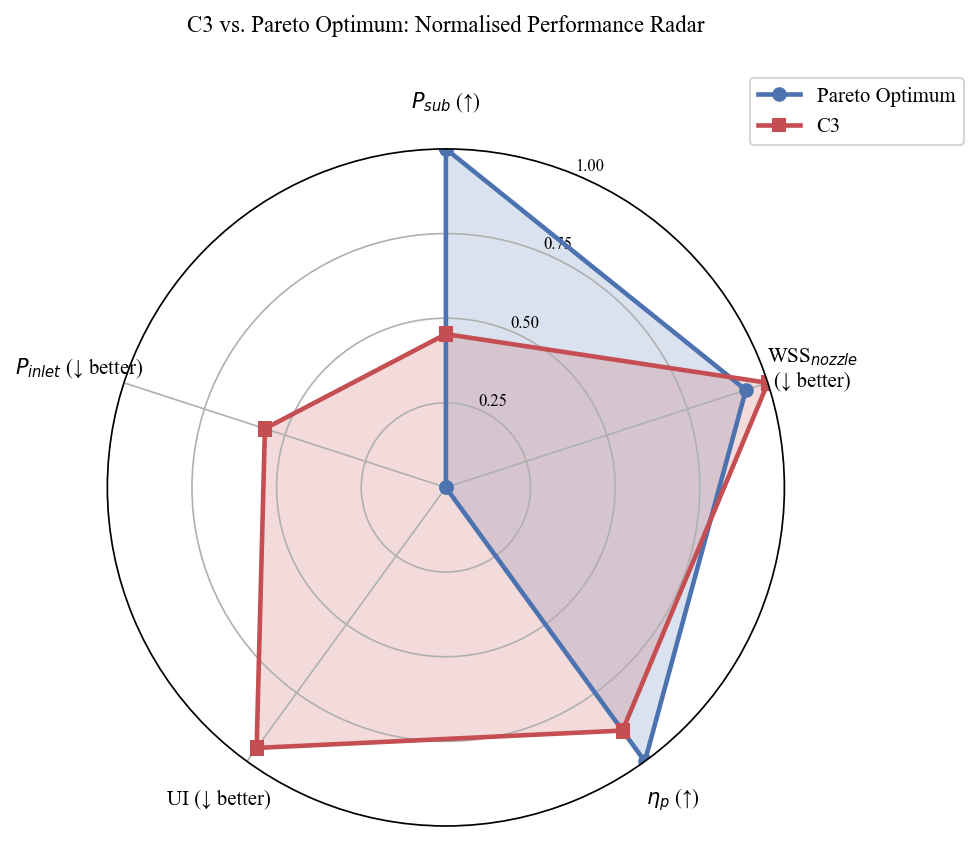
\includegraphics[width=0.7\textwidth]{figures/5.8.png}
  \caption{NSGA-II验证工况与C3对比雷达图}
  \label{fig:5.8}
\end{figure}

对比两项试验结果，有以下几个角度值得讨论：

（1）压实效果：NSGA-II最优工况的$P_{sub,AWA} = 43760$~Pa，较C3（21702~Pa）提升+102\%，几乎翻倍。这一巨大提升主要来自两方面：$\alpha = 14.06°$与$TL = 70$~mm将层高压缩至5~mm，楔形效应达到最大，且$TL$的增大进一步延长了约束路径，两者协同产生了极高的接触压力。

（2）泵送能耗：接触压力翻倍，泵送压力也近乎翻倍。NSGA-II最优工况的$P_{inlet} = 73844$~Pa，较C3（38772~Pa）增加+90\%，几乎同比例上升。结合\cref{eq:Pinlet-Psub}所揭示的$P_{inlet} \approx 1.42 \times P_{sub}$共线关系，可以完全解释这一现象。

（3）压力传递效率：NSGA-II最优工况的$\eta_p = 0.593$，较C3的0.560仅提升+5.9\%。这一结果说明最优工况花费90\%更多的泵送能耗，但是仅仅只能换来5.9\%的效率改善。从投入产出比的角度来看，追求比C3更高的接触压力的边际效益极低，工程代价极高。

（4）层高：NSGA-II最优工况是课题研究设置的最低值，而这个结果本身就会带来一定的不确定性：如果为了极限优化的其它目标而去压榨最终打印混凝土的层高，那么混凝土层高本身作为一个打印混凝土结果中重要的评价指标，它的不确定性将会大大增加。一旦出现材料流变性能波动或设备误差，极易导致整形板末端与已打印层发生接触，破坏打印质量。

综合以上分析可以得出：NSGA-II最优解代表了本研究参数范围内的理论压实极限，但其高达73844~Pa的泵送压力要求以及极小的层高余量，使其在工程实践中的可行性受到严格限制。C3工况（$P_{sub} = 21702$~Pa，$P_{inlet} = 38772$~Pa，$H = 6.47$~mm）在保持合理泵送压力和充足层高余量的前提下，实现了相对于基准工况161\%的压实提升，是综合性能与工程可靠性的最优平衡点，也是本研究推荐的工程实用方案。
